% split code (latex) parts into different files

% enhance listings

% "Deep Learning for Time Series Forecasting" by Jason Brownlee

% RNNs (Recurrent Neural Networks) (можно чуть чуть написать и сказать, что затронем 
% подробнее в следующей главе)

% LSTM (Long Short-Term Memory) (может пока не трогать, тк это модификация RNN)

% GRU (может пока не трогать, тк это модификация RNN)

% -------------

% topological intuition behind NN
% talk about backpropagation 
% universal approximation theorem (from Goodfellow)
% Manifold learning
% intuition behind thinking in n dimensions
% sigmoid/relu/softmax e.t.c. discussion for which is better
% parallel to neurobilogy
% architecture definition, main terms
% feed forward/not feed forward
% talk about gradient descent (stohastic, adam?)
% bayessian statistics? how is it different from classic 
% the idea of deriving cost functions from maximum likelihood
% maximum likelihood
% no free lunch theorem
% Regularization
% SVM and kernel trick
% cross entropy and Kullback–Leibler divergence

% --------------

% https://chatgpt.com/c/6817eeff-5420-8010-b35d-3c35fed4bdcf
% https://aistudio.google.com/prompts/1akCvM2Z46N9sApnbcqEbhtnS8eMy7HLz

% Part 1: Setting the Stage - What are we trying to do?
%     Introduction to Machine Learning & Supervised Learning

%     Intuition behind Thinking in n Dimensions

%     maybe drop:
%     (SVM & the kernel trick (how it bends space (later will be compared to nonlinearity in activation functions)))

%     What Is a Neural Network?
%     - Parallel to neurobiology
%     - Architecture definitions & main terms
%     - Feed‑forward vs. recurrent    

% Part 2: How Neural Networks "Compute"
%     How NNs “Fire”
%     - Activation functions(Sigmoid/ReLU/Softmax etc.):
%     (show how each nonlinearity “folds” space)
        
%     Geometric & Topological Intuition
%     - Manifold learning (quick review, mainly for intuition)
%     - topological intuition behind NN

% Part 3: How Neural Networks Learn
%     Cost functions (MSE, cross-entropy)

%     Probabilistic loss
%     - maximum likelihood 
%     - Deriving Cost Functions from Maximum Likelihood
%     (Cross‑entropy & Kullback–Leibler divergence (note: cross‑entropy ↔ KL divergence & MLE in one bullet))

%     Gradient descent mechanism (closed optimization, convex, e.t.c.)
%     Backpropagation
%     Optimization landscapes: local minima vs. saddle points (intuition).
%     Gradient Descent Variants (Stochastic, Mini-batch, Adam)

% Part 4: Theoretical & Practical Considerations
%     Universal Approximation Theorem
%     Overfitting and Underfitting
%     Regularization
%     Training, Validation, and Test Sets (hyperparameter tuning)
%     No Free Lunch Theorem

% Part 5: Bridging to RNNs
%     Limitations of Feed-Forward Networks for Sequences

% --------------

% Dimensionality reduction and visualisation of high dimensional data (https://colah.github.io/posts/2014-10-Visualizing-MNIST/)
% t-SNE

% \section{Рекуррентные нейронные сети}
\section{Глубокие сети}

Глубокие сети прямого распространения, которые называют также нейронными
сетями прямого распространения, или многослойными перцептронами (МСП), -
самые типичные примеры моделей глубокого обучения. Цель сети прямого расп­рост­ранения 
- аппроксимировать некоторую функцию $f^*$. Например, в случае классификатора 
$y = f^*(\bm{x})$ отображает вход $\bm{x}$ в категорию $y$. Сеть прямого распространения
определяет отображение $y = f(\bm{x}; \bm{\theta})$ и путем обучения находит 
значения параметров $\bm{\theta}$, дающие наилучшую аппроксимацию.

\subsection{Что такое нейронная сеть? {\color{red} todo}}

В данной главе кратко вводятся основные понятия глубокого обучения. 
Чтобы понять, как нейронные сети обрабатывают информацию, 
полезно сначала рассмотреть, как мы представляем данные, 
с которыми они работают. Часто эти данные существуют в многомерных пространствах, 
поэтому мы сначала сформулируем методы мышления в этих пространствах.
Затем рассмотрим модель перцептрона и закончим данную главу ознакомлением с 
архитектурой многослойного перцептрона (MLP), 
определив все, сопутствующие ему, основные термины.

Предполагается, что читатель уже знаком с основами классического машинного обучения, 
поэтому мы не будем подробно останавливаться на соответствующих понятиях.

\subsubsection{Интуиция мышления в n измерениях}

В процессе эволюции люди научились рассуждать в двух и трех измерениях. 
Приложив достаточно усилий, мы можем мыслить и в четырех измерениях. 
Машинное обучение часто требует от нас работы с тысячами измерений - 
или десятками тысяч, или миллионами. Даже очень простые вещи становится 
трудно понять, когда вы делаете их в очень большом количестве измерений.

Поэтому важно иметь в запасе методы для работы с такими данными. 
Люди, которые научились хорошо мыслить в высоких измерениях часто 
распологают, своего рода, ментальной библиотекой, содержащей множество 
различных техник. Возможно, эти техники не выделяются простотой, 
к которой мы привыкли при визуализации трех измерений, но, 
собрав библиотеку таких техник, вы сможете довольно хорошо научиться 
мыслить в высоких измерениях.

Рассмотрим несколько таких техник \cite{ndim_thinking}:

\begin{quoting}
    \itshape
    “Можно рассматривать высокоразмерное векторное пространство как 
    пространство состояний для системы со многими степенями свободы. 
    Например, мегапиксельное изображение - это точка в миллионном 
    векторном пространстве; изменяя изображение, можно исследовать 
    это пространство, и различные подмножества этого пространства 
    соответствуют различным классам изображений.

    Аналогичным образом можно интерпретировать звуковые волны, 
    коробку с газами, экосистему, совокупность избирателей, поток 
    цифровых данных, испытания случайных величин, результаты 
    статистического исследования, вероятностную стратегию в игре 
    двух игроков и многие другие конкретные объекты как состояния 
    в высокоразмерном векторном пространстве, а различные базовые 
    понятия, такие как выпуклость, расстояние, линейность, смена 
    переменных, ортогональность или внутреннее произведение, могут 
    иметь вполне естественные значения в некоторых из этих моделей 
    (хотя и не во всех).“
\end{quoting}

\begin{quoting}
    \itshape
    “Если вы пытаетесь представить себе некое 4D явление $P$, 
    сначала подумайте о соответствующем 3D явлении $P'$, 
    а затем представьте себя в роли 2D существа, которое 
    пытается представить себе $P'$. Преимущество в том, что, в отличие 
    от случая 4D vs. 3D, вы сами можете легко переключаться между 3D 
    и 2D перспективами и, следовательно, можете получить представление 
    о том, какая именно информация теряется, когда вы опускаете измерение. 
    (Можно назвать это «трюком Флатландии» ("Flatland trick"), в честь самого 
    известного литературного произведения, опирающегося на данную идею).“
\end{quoting}

Нейронные сети оперируют именно с такими многомерными представлениями данных, 
преобразуя их для решения поставленных задач.

\subsubsection{Нейронная сеть}

Нейронные сети, как можно догадаться из названия, были вдохновлены работой человеческого 
мозга. Идея использовать несколько слоев векторных представлений пришла из нейробиологии. 
Выбор функций, используемых для расчета этих представлений был также навеян 
экспериментально полученными фактами о функциях, вычисляемых биологическими нейронами. 
Современные исследования в области нейронных сетей, однако, руководствуются 
многими математическими и инженерными дисциплинами, и у них нет цели идеально 
смоделировать работу мозга. О сетях прямого распространения лучше думать 
не как р моделях функционирования мозга, а как о 
механизмах для аппроксимации функций, спроектированных с целью достижения 
статистического обобщения, периодически вдохновляемых нашими знаниями о работе 
мозга.

\paragraph{Перцептрон}

Нейронная сеть (neural network) строится из простейших элементов - искусственных 
нейронов. Одной из первых моделей такого нейрона был перцептрон, 
предложенный Фрэнком Розенблаттом в 1958 году \cite{Rosenblatt_perceptron}. Несмотря на то, что в 
современных архитектурах чаще используют сигмоидальные и ReLU-нейроны, 
понимание перцептрона важно для осознания эволюции подходов к обучению 
и архитектуре сетей.

Так как работает модель перцептрона? Перцептрон принимает на вход несколько бинарных значений: 
$x_1, x_2, ..., x_n $ и возвращает единственное бинарное значение:

\begin{figure}[h!]
    \centering
    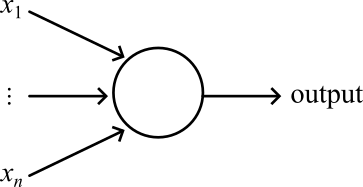
\includegraphics[width=0.4\textwidth, keepaspectratio]{perceptron}
    \caption{Модель перцептрона.}
    \label{fig:perceptron}
\end{figure}

Розенблатт предложил простую идею для расчета выходного значения. Он ввел понятие 
весов $w_1, w_2, ..., w_n$, действительных значений, отражающих важность каждого из, 
соответствующих входов. Выходное значение нейрона определяется из правила, превышает 
ли взвешенная сумма входов некоторое наперед заданное значение, называемое порогом 
(threshold):

\begin{equation*}
    \text{output} = \begin{cases}
        0 \quad \text{if} \quad \sum_j w_j x_j \leq \text{threshold} \\
        1 \quad \text{if} \quad \sum_j w_j x_j > \text{threshold} 
    \end{cases}
\end{equation*}

Однако, в машинном обучении чаще используют упрощенную версию данной записи. 
Перепишем $\sum_j w_j x_j$ в виде скалярного произведения, \hspace{20pt}
$\bm{w} \cdot \bm{x} \equiv \sum_j w_j x_j$, 
а порог заменим смещением (bias), $b \equiv -\text{threshold}$. Тогда наша запись примет вид:

\begin{equation*}
    \text{output} = \begin{cases}
        0 \quad \text{if} \quad \bm{w} \cdot \bm{x} + b \leq 0 \\
        1 \quad \text{if} \quad \bm{w} \cdot \bm{x} + b > 0 
    \end{cases}
\end{equation*}

Одним из примеров применения перцептрона может послужить вычисление логических функций.
Так, например, рассмотрим перцептрон, у которого всего два входа, $x_1, x_2 \in \left\{ 0, 1 \right\}$. 
И вручную примем $w_1 = w_2 = -2, \quad b = 3$. Тогда наш перцептрон примет вид:

\begin{figure}[h!]
    \centering
    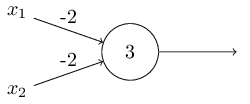
\includegraphics[width=0.4\textwidth, keepaspectratio]{perceptron2}
    \caption{Пример перцептрона с весами $\bm{w} = \left[ -2 \hspace{3pt} -2 \right]^T$ и 
    смещением $b = 3$.}
    \label{fig:perceptron2}
\end{figure}

При $\bm{x} = \left[ 0 \hspace{3pt} 0 \right]^T$, получим $1$, т.к. 
$\bm{w} \cdot \bm{x} + b = (-2) \cdot 0 + (-2) \cdot 0 + 3 = 3 > 0$.
Построим таблицу всех значений:

\begin{minipage}{0.4\textwidth}
    \centering
    \renewcommand{\arraystretch}{1.5}
    \begin{tabular}{ccc}
        $x_1$ & $x_2$ & $f$ \\
        \midrule
        0 & 0 & 1 \\
        0 & 1 & 1 \\
        1 & 0 & 1 \\
        1 & 1 & 0 \\
    \end{tabular}
    \captionof{table}{Значения, которые принимает перцептрон (\ref{fig:perceptron2}) 
    при различных значениях $x_1, x_2 \in \left\{ 0, 1 \right\}$.}
    \label{tab:perceptron-values}
\end{minipage}
\hspace{30pt}
\begin{minipage}{0.4\textwidth}
    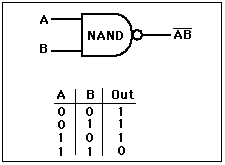
\includegraphics[width=\linewidth]{NAND}
    \captionof{figure}{Штрих Шеффера (NAND gate).}
    \label{fig:NAND}
\end{minipage}\\

Таким образом, наш перцептрон реализует Штрих Шеффера (NAND gate). 
Исходя из этого примера видно, что мы можем использовать перцептроны для 
расчета простых логических функций. Вообще говоря, мы можем рассчитать любую логическую 
(и не только, см. {\color{red} главу...}) функцию, 
используя сеть из перцептронов, называемаю нейронной сетью.

\paragraph{Архитектура нейронной сети}

Нейронная сеть состоит из композиции нейронов (т.е. когда в качестве входов для 
нейронов используются выходы других нейронов), например:

\begin{figure}[h!]
    \centering
    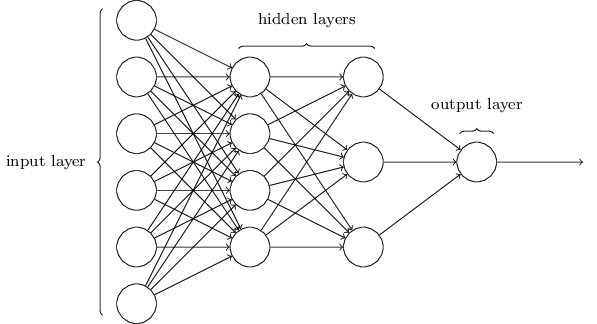
\includegraphics[width=0.8\textwidth, keepaspectratio]{NN_example1}
    \caption{Архитектура простой нейронной сети.}
    \label{fig:NN1}
\end{figure}

Самый левый слой называется \textit{входным слоем (input layer)}, а нейроны в нем 
называются \textit{входными нейронами (input neurons)}. Самый правый, или же 
\textit{выходной слой (output layer)} содержит в себе 
\textit{выходные нейроны (output neurons)}. Слои между ними называются 
\textit{скрытыми (hidden layers)}. Количество скрытых слоев определяет 
\textit{глубину (depth)} нейронной сети, а размерность скрытых слоев 
определяет \textit{ширину (width)} модели.

Подобные сети называют \textit{многослойными перцептронами (MLPs)}. (Исторически пошло, 
что иногда их так называют даже когда они состоят не из перцептронов). 

\paragraph{feedforward vs recurrent}

До сих пор мы обсуждали нейронные сети, в которых выход из одного слоя используется как 
вход для следующего. Подобные сети называются \textit{нейронными сетями прямого распространения 
(feedforward neural networks)}. Это значит, что у нас нет циклов в сети - информация всегда 
поступает вперед и никогда не возвращается назад.

Однако существуют и другие модели искусственных нейронных сетей, 
в которых возможны циклы обратной связи. Подобные модели называются 
\textit{рекуррентными нейронными сетями (recurrent neural networks)} 
(см. {\color{red} главу...}). 
Идея этих моделей заключается в 
том, что нейроны работают в течение некоторого ограниченного периода 
времени, а затем затихают. Это возбуждение может стимулировать другие 
нейроны, которые через некоторое время также возбуждаются на ограниченное 
время. Это заставляет еще большее количество нейронов срабатывать, и 
так со временем мы получаем каскад нейронов, которые срабатывают. Циклы 
в такой модели не вызывают проблем, так как выход нейрона влияет на его 
вход только через некоторое время, а не мгновенно \cite{NN_Nielsen}.

\subsection{Как нейронные сети «вычисляют»?}

\textit{Функции активации} в нейронной сети задают правило преобразования 
взвешенной суммы входа в выход. Простейший пример функции активации мы уже 
рассмотрели на примере перцептрона, однако в силу своей простоты, он не очень 
эффективен. 

Выбор функции активации оказывает огромное виляние на возможности и производительность 
нейронной сети, и различные функции активации могут быть использованы в раличных частях модели.

Как правило, всем скрытым слоям назначают одну и ту же функцию активации, 
а функция активации выходного слоя, как правило, отличается и подбирается в 
зависимости от типа решаемой задачи.

Функции активации также обычно дифференцируемы, то есть производная первого порядка 
может быть вычислена для заданного входного значения. Это необходимо, учитывая, что 
нейронные сети обычно обучаются с помощью алгоритма обратного распространения ошибки 
(см. главу {\color{red} todo}), 
который требует производной ошибки прогнозирования для обновления весов модели.

Существует множество различных функций активациии, но на практике используется не 
так много. Вообще говоря, многие дифференцируемые функции показывают отличные результаты. 
Есть целый ряд неопубликованных функций активации, которые ведут
себя ничуть не хуже популярных, однако в ходе исследований обычно 
обнаруживается, что результаты, полученные при отходе от стандартной практики, 
вполне сопоставимы. Это означает, что новые типы скрытых блоков
обычно публикуются только в случае, когда улучшение весомо и очевидно. Скрытые
блоки, работающие примерно так же, как известные, - дело настолько обычное, что
рассматривать их неинтересно.

\subsubsection{Функции активации}

До сих пор, мы подбирали параметры вручную. Однако, у нас возникли бы серьезные 
проблемы, если бы мы захотели подобрать параметры к, например, следующей нейронной сети:

\begin{figure}[h!]
    \centering
    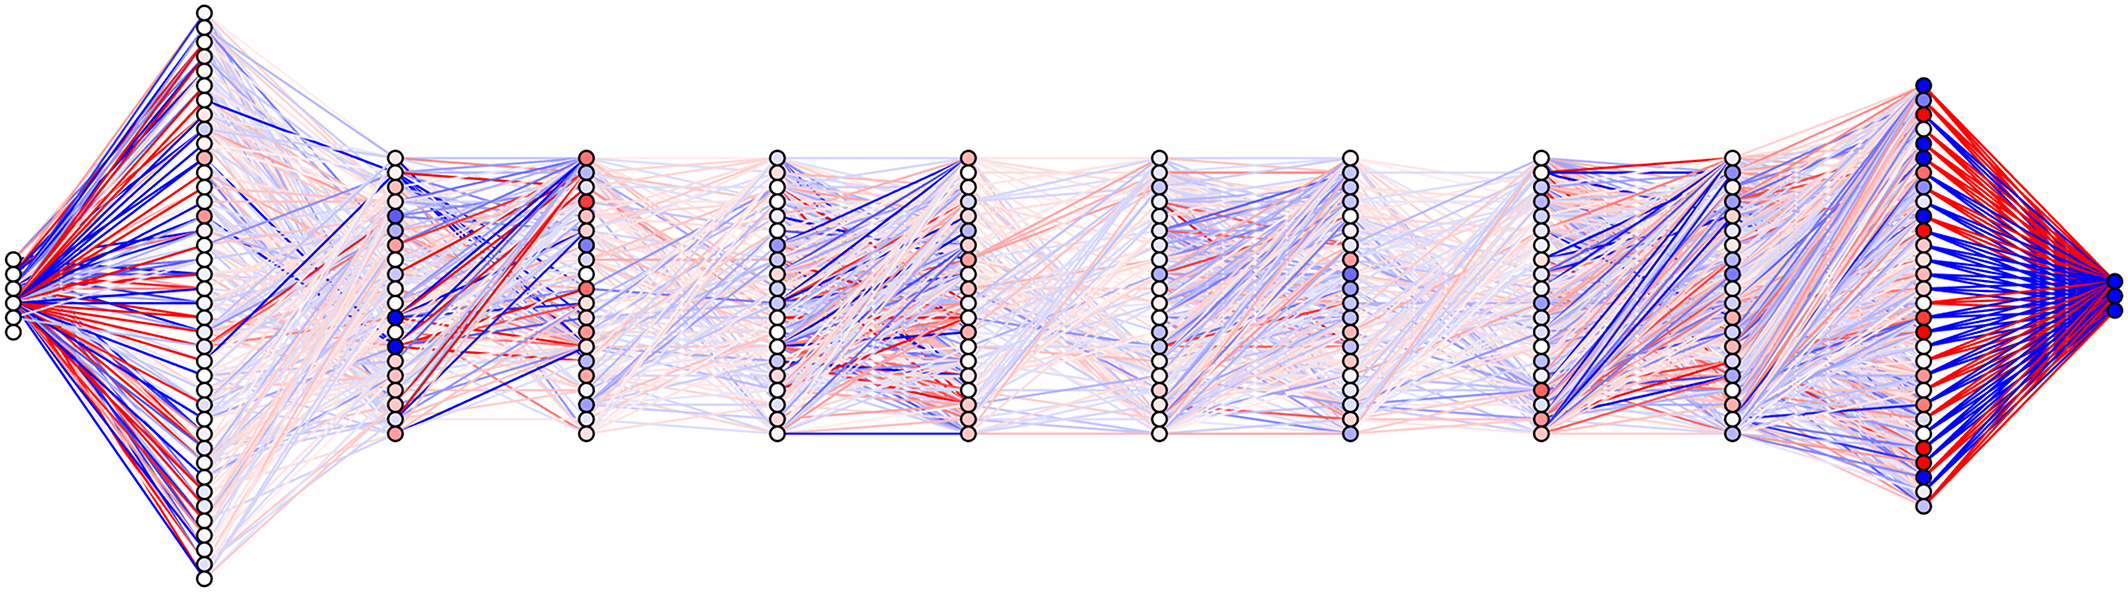
\includegraphics[width=1\textwidth, keepaspectratio]{NN_example3}
    \caption{Архитектура нейронной сети.}
    \label{fig:NN3}
\end{figure}

Которая, вообще говоря, считается относительно небольшой по современным меркам 
(ходят слухи, что модель GPT-4 насчитывает $\sim 1.8$ триллионов параметров в 
120 слоях \cite{gpt4_architecture}).

Однако ситуация лучше, чем кажется на первый взгляд. 
Проектирование и обучение нейронной сети не сильно отличается от обучения 
любой другой модели машинного обучения с помощью градиентного спуска. 

Таким образом, мы возвращаеся к проблеме перцептронов с жёсткой (ступенчатой) 
функцией активации:
\begin{equation*}
    \text{output} = \begin{cases}
        0 \quad \text{if} \quad \bm{w} \cdot \bm{x} + b \leq 0 \\
        1 \quad \text{if} \quad \bm{w} \cdot \bm{x} + b > 0 
    \end{cases}
\end{equation*}

Хотя такая модель достаточно проста, её основное ограничение в том, 
что функция активации не является дифференцируемой в точке разрыва, 
а её производная равна нулю везде, где она определена. 
Из-за этого градиентный спуск применять невозможно: градиент отсутствует или 
обращается в ноль, и веса не обновляются.

\paragraph{Сигмоидальные блоки}

На помощь приходит новый вид искусственных нейронов, называемый 
\textit{сигмоидальным (sigmoid neuron)} (далее будем называть просто сигмоидом). 
Основное отличие от перцептрона заключается в том, что
сигмоид может вернуть любое значение из интервала от 0 до 1, 
задаваемое гладкой, непрерывно дифференцируемой функцией $\sigma$, 
называемой сигмоидальной функцией:
\begin{equation*}
    \sigma(z) \defeq \cfrac{1}{1 + e^{-z}}
\end{equation*}

Таким образом функция активации принимает вид:
\begin{equation*}
    \text{output} = \sigma(\bm{wx} + b) = \cfrac{1}{1 + e^{-\bm{wx} - b}}
\end{equation*}

Если мы посмотрим на графики функций активации перцептрона и сигмоида, то 
заметим, что сигмоидальная функция это просто сглаженная версия ступенчатой 
(Вообще говоря, при $\bm{wx + b = 0}$ перцептрон возвращает 0, а ступенчатая 
функция 1. Так что строго говоря ступенчатую функцию следовало бы изменить в 
этой одной точке, чтобы ее можно было называть функцией активации перцептрона, но 
суть понятна).

\begin{minipage}{0.4\textwidth}
    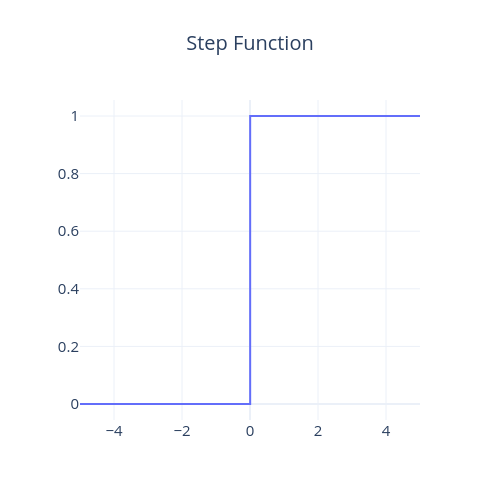
\includegraphics[width=\linewidth]{step}
    \captionof{figure}{График ступенчатой функции.}
    \label{fig:step}
\end{minipage}
\hspace{30pt}
\begin{minipage}{0.4\textwidth}
    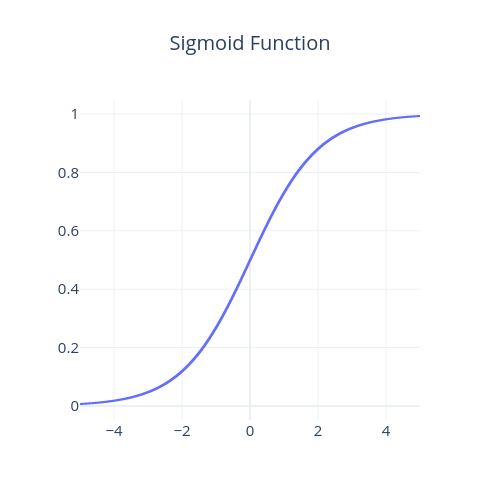
\includegraphics[width=\linewidth]{sigma}
    \captionof{figure}{График сигмоидальной функции.}
    \label{fig:sigma}
\end{minipage}\\

Иногда вместо сигмоидальной функции используют гиперболический тангенс\\ 

\begin{minipage}{0.4\textwidth}
    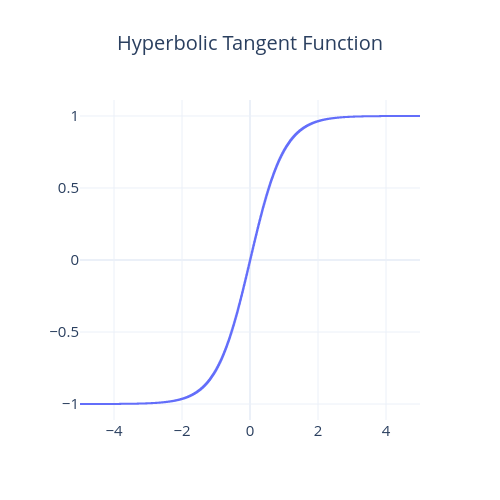
\includegraphics[width=\linewidth]{tanh}
    \captionof{figure}{График гиперболического тангенса.}
    \label{fig:tanh}
\end{minipage}
\hspace{30pt}
\begin{minipage}{0.3\textwidth}
    \begin{equation*}
        \text{tanh}(z) \defeq \cfrac{e^{2z} - 1}{e^{2z} + 1}
    \end{equation*}
\end{minipage}\\

Эти функции активации тесно связаны: $\text{tanh}(z) = 2 \sigma(2z) - 1$.

Однако, сигмоидальные блоки близки к асимптоте в большей части своей области определения -
приближаются к высокому значению, когда $z$ стремится к бесконечности, и к низкому,
когда $z$ стремится к минус бесконечности. Высокой чувствительностью они обладают 
только в окрестности нуля. Из-за насыщения сигмоидальных блоков градиентное
обучение сильно затруднено. Поэтому использование их в качестве скрытых блоков
в сетях прямого распространения ныне не рекомендуется. Применение же в качестве
выходных блоков совместимо с обучением градиентными методами, если функция
стоимости компенсируется насыщением сигмоиды в выходном слое.

Сигмоидальные функции активации все же применяются, но не в сетях прямого
распространения. К рекуррентным сетям, многим вероятностным моделям и некоторым 
автокодировщикам предъявляются дополнительные требования, исключающие
использование кусочно-линейных функций активации и делающие сигмоидальные
блоки более подходящими, несмотря на проблемы насыщения.

\paragraph{Блоки линейной ректификации}

В качестве функции активации по умолчанию для большинства нейронных сетей прямого 
распространения рекомендуется ректифицированная линейная функция активации (ReLU):

\begin{minipage}{0.45\textwidth}
    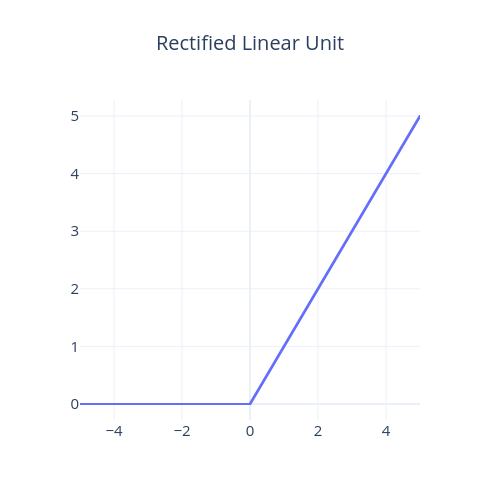
\includegraphics[width=\linewidth]{ReLU}
    \captionof{figure}{График ректифицированной линейной функции.}
    \label{fig:ReLU}
\end{minipage}
\hspace{30pt}
\begin{minipage}{0.2\textwidth}
    \begin{align*}
        \text{ReLU}(z) &= z^{+} \\
        &= \text{max}(0, z) \\
        &= \cfrac{z + |z|}{2} \\[0.5em]
        &= \begin{cases}
            z \quad \text{if} \quad z > 0, \\
            0 \quad \text{if} \quad z \leq 0
        \end{cases}
    \end{align*}
\end{minipage}\\

Применение ее к выходу линейного преобразования дает нелинейное преобразование. 
Функция, впрочем, очень близка
к линейной - она является кусочно-линейной с двумя линейными участками. 
Поскольку блоки линейной ректификации почти линейны, сохраняются
многие свойства, благодаря которым линейные модели легко поддаются
оптимизации градиентными методами. Сохраняются также свойства, обес­печивающие 
хорошую обобщаемость линейных моделей. Общий принцип
информатики - строить сложные системы из минимальных компонентов.
От памяти машины Тьюринга требуется только способность хранить нуль
и единицу, а универсальный аппроксиматор можно построить из ректифи-
цированных линейных функций \cite{Goodfellow-et-al-2016}.

\paragraph{Нелинейность}

После того как мы познакомились с различными функциями активации, 
возникает естественный вопрос: зачем вообще нужны эти нелинейные функции активации? 
Почему бы не использовать простые линейные функции? 
Ведь их так легко оптимизировать методом градиентного спуска. 
К сожалению, дело в том, что композиция любых линейных преобразований остаётся линейной 
функцией входа, а значит и вся сеть прямого распространения остается линейной 
функцией входа.

Пусть у нас есть две кривые линии на плоскости и задача нейронной сети заключается в том, 
чтобы классифицировать к которой из двух кривых принадлежит та или иная точка. В случае 
линейной модели, мы бы не добились особого успеха, тк наши кривые линейно неразделимы:\\

\begin{minipage}{0.35\textwidth}
    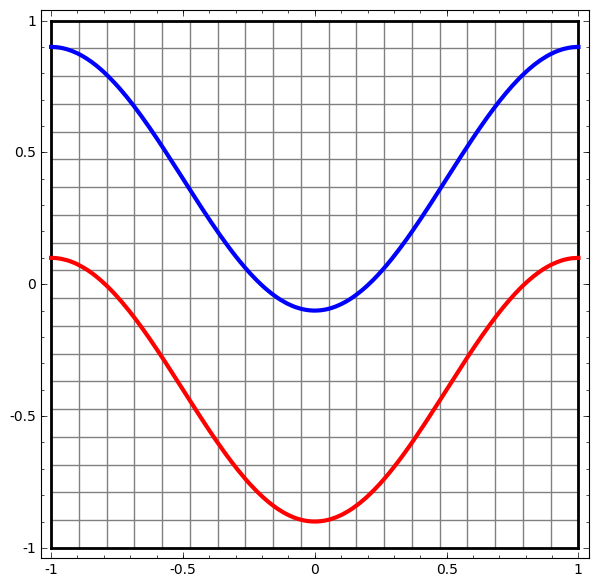
\includegraphics[width=\linewidth]{colah1}
    \captionof{figure}{}
    \label{fig:colah1}
\end{minipage}
\hspace{80pt}
\begin{minipage}{0.35\textwidth}
    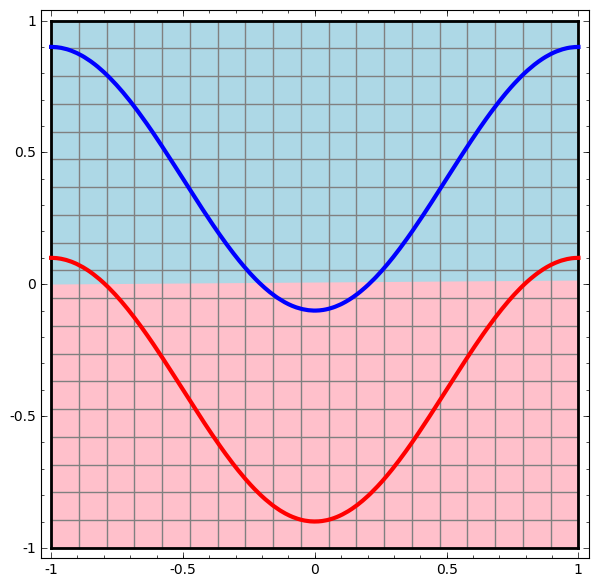
\includegraphics[width=\linewidth]{colah2}
    \captionof{figure}{}
    \label{fig:colah2}
\end{minipage}\\

Однако, если перед классификацией, мы преобразуем наши данные 
(в данном случае, с применением сигмоидальной функции), 
то получим их \textit{представление (representation)} в 
пространстве, в котором их уже легче классифицировать \cite{colah}:

\begin{figure}[h!]
    \centering
    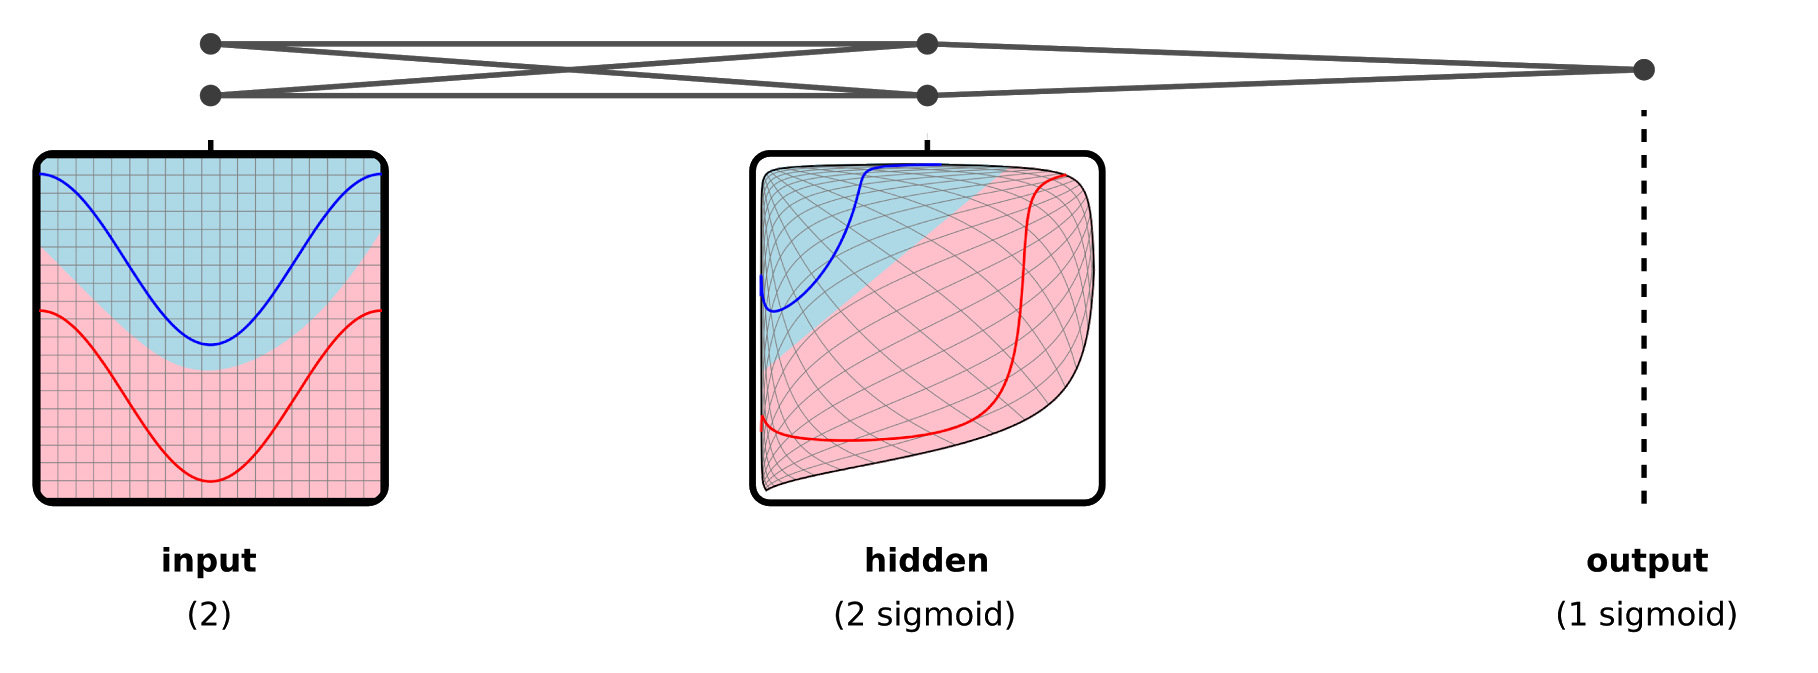
\includegraphics[width=1\textwidth, keepaspectratio]{colah3}
    \caption{Иллюстрация того, как нелинейный слой «разворачивает» 
    данные в новом пространстве признаков, делая их линейно разделимыми.}
    \label{fig:colah3}
\end{figure}

Таким образом, каждый слой с нелинейной активацией потенциально «перестраивает» или 
«разворачивает» пространство признаков, делая сложные зависимости более явными для 
последующих слоев или для финального классификатора.

\subsubsection{Многообразия и топология {\color{red} todo}}

% leave for later

% Placement: This could fit well after the "Нелинейность" paragraph and the 
% Colah visualization.

% Content (Keep it Intuitive):

%     "Данные, с которыми мы работаем (например, изображения, звуки), 
%     хоть и представлены в пространствах высокой размерности, 
%     часто лежат на структурах меньшей размерности, называемых 
%     многообразиями (manifolds)." (Think of a rolled-up sheet of 
%     paper in 3D space – the paper itself is 2D).

%     "Задача нейронной сети, с этой точки зрения, – научиться 'разворачивать' 
%     эти сложные многообразия или преобразовывать их так, чтобы интересующие 
%     нас классы или закономерности стали легко отделимы (например, линейно отделимы)."

%     "Нелинейные функции активации и многослойная архитектура как раз и 
%     позволяют сети выполнять такие сложные топологические преобразования 
%     пространства признаков."

%     Avoid deep math. Focus on the idea of "simplifying the data's geometry."

\subsection{Как нейронные сети обучаются?}

Теперь, когда мы понимаем устройство нейронной сети, возникает вопрос: 
как подобрать её параметры (веса и смещения) так, чтобы она решала нужную нам задачу? 
Из машинного обучения известно, что данный процесс называется обучением модели и требует 
способа измерить насколько хорошо модель справляется с задачей на имеющихся у нас данных. 
Эту роль выполняет \textit{функция стоимости (или функция потерь)}.

\subsubsection{Функции стоимости}

Большинство современных нейронных сетей обучают с применением метода максимального 
правдоподобия. То есть функция стоимости это просто отрицательное логарифмическое 
правдоподобие, которое можно эквивалентно описать как перекрестную энтропию 
между обучающими данными и распределением модели. Подобная функция стоимости 
задается формулой 
\begin{equation*}
    J(\theta) = - \mathbb{E}_{\bm{x},\bm{y} \sim \hat{p}_{\text{data}}} \text{log} \left[ p_\text{model} (\bm{y} | \bm{x}) \right].
\end{equation*}

Интуитивно, минимизация такой функции стоимости эквивалентна поиску таких параметров 
модели, при которых наблюдаемые нами данные были бы наиболее «вероятны» с точки 
зрения модели.

Конкретная форма функции стоимости меняется от модели к модели в зависимости от выбранной 
формы $\text{log} \left[ p_\text{model} \right]$. Раскрытие этой формулы обычно дает члены, которые не
зависят от параметров модели и могут быть отброшены. Например если принять 
$p_\text{model}(\bm{y} | \bm{x}) = N(\bm{y}; f(\bm{x}; \bm{\theta}), \bm{I})$, то 
мы получим знакомую среднеквадратическую ошибку (MSE):
\begin{equation*}
    J(\theta) = \cfrac{1}{2} \mathbb{E}_{\bm{x},\bm{y} \sim \hat{p}_{\text{data}}} || \bm{y} - f(\bm{x}; \bm{\theta}) ||^2 + \text{const}.
\end{equation*}

с точностью до масштабного коэффициента $\frac{1}{2}$ и члена, не зависящего от 
$\bm{\theta}$. 

Преимущество такого подхода - вывода функции стоимости из оценки максимального 
правдоподобия - в том, что отпадает необходимость проектировать функцию 
стоимости заново для каждой модели. Задание модельного распределения $p(\bm{y} | \bm{x})$ 
автоматически определяет функцию стоимости $\text{log} \left[ p(\bm{y} | \bm{x}) \right]$ 
\cite{Goodfellow-et-al-2016}.

\subsubsection{Метод обратного распространения ошибки}

Метод обратного распространения ошибки (backpropagation, далее backprop) это 
эффективный способ вычисления градиента при обучении глубоких нейронных сетей. 
Вообще говоря это ключевый алгоритм, который сделал обучение глубоких моделей 
вычислительно возможным. Для современных нейронных сетей, в некоторых случаях, 
он позволяет ускорить обучение методом градиентного спуска в 10 миллионов раз, по 
сравнению с наивным подходом (для сравнения, это разница между тем, что модель 
обучается неделю и 200 000 лет). 

Backprop не эксклюзивен для глубокого обучения, этот мощный вычислительный 
инструмент используют и во многих дургих областях, просто под другим названием. 
В общем случае алгоритм носит название «Reverse mode automatic differentiation».

\paragraph{Предпосылка}

В основе алогритма лежит правило дифференцирования сложной функции 
(Chain Rule of Calculus), которое мы последовательно используем для 
расчета производных функций, сформированных композицией других функций, чьи 
производные мы уже знаем.

С использованием backprop, обучение нейронной сети происходит в два этапа:

\textbf{Прямое распространение (Forward Propagation):} 
Во время прямого распространения, NN пытается
угадать лучший, возможный на текущий момент, результат. 
Для этого она пропускает входные данные через 
каждый свой слой.

\textbf{Обратное распространение (Backward Propagation):} 
Во время обратного распространения, NN
подстраивает свои параметры, пропорционально ошибке, полученной из попытки
угадывания. Она это делает, перемещаясь обратно от результата, собирая
производные ошибки по отношению к параметрам функции (градиенты), и
оптимизируя параметры с помощью градиентного спуска.

\paragraph{Вычислительный граф}

Концептуально, математические выражения удобно рассматривать в виде 
вычислительных графов. Допустим у нас есть некоторое выражение $f$, 
составленное из переменных $a, b, c$:
\begin{equation*}
    f = 3a + b^2 - c^a
\end{equation*}

Введем для удобства еще две переменные $d, e$:
\begin{gather*}
    d = 3 \cdot a + b^2 \\
    e = c^a \\
    f = d - e
\end{gather*}

Тогда вычистельный граф данного выражения можно представить в виде:
\begin{figure}[h!]
    \centering
    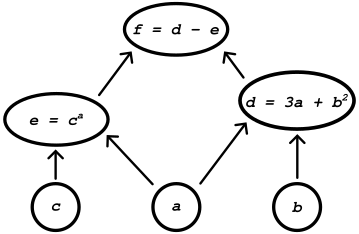
\includegraphics[width=0.5\textwidth, keepaspectratio]{backprop_graph_forward}
    \caption{Вычислительный граф выражения $f = 3a + b^2 - c^a$, разбитого на две 
    дополнительные части: $e = c^a$ и $d = 3a + b^2$. $a, b, c$ - переменные.}
    \label{fig:backprop_graph_forward}
\end{figure}

% \begin{tikzpicture}[
%     >=latex,
%     node distance=2cm,
%     thick,                             % make all lines bolder
%     every circle/.style={minimum size=1cm},           % all circles at least 1cm diameter
%     every ellipse/.style={minimum width=3cm, minimum height=1cm}
%   ]
%   % bottom layer: input circles
%   \node[draw,circle] (c) at (0,0) {$c$};
%   \node[draw,circle] (a) at (3,0) {$a$};
%   \node[draw,circle] (b) at (6,0) {$b$};

%   % middle layer: ellipses
%   \node[draw,ellipse] (e) at (1,2) {$e = c^a$};
%   \node[draw,ellipse] (d) at (5,2) {$d = 3a + b^2$};

%   % top layer: ellipse
%   \node[draw,ellipse] (f) at (3,4) {$f = d - e$};

%   % arrows
%   \draw[->] (c) -- (e);
%   \draw[->] (a) -- (e);
%   \draw[->] (a) -- (d);
%   \draw[->] (b) -- (d);
%   \draw[->] (e) -- (f);
%   \draw[->] (d) -- (f);
% \end{tikzpicture}

\newpage
Выбрав определенные значения для $a, b, c$ мы можем вычислить чему будует равно 
наше выражение $f$:
\begin{figure}[h!]
    \centering
    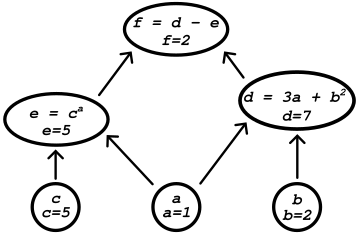
\includegraphics[width=0.5\textwidth, keepaspectratio]{backprop_graph_forward_eval}
    \caption{Вычислительный граф выражения, изображенного на рис. 
    \ref{fig:backprop_graph_forward}, вычисленного при $a=1, b=2, c=5$.}
    \label{fig:backprop_graph_forward_eval}
\end{figure}

Таким образом мы произвели прямой проход по графу (прямое распространение): 
от входных значений к выходному. Достигнув нашей вершины графа, мы 
теперь можем развернуть направление стрелок и пройтись в обратном направлении 
(обратное распространение), считая частные производные. В конечном итоге мы получим 
производную $f$ относительно всех узлов:

\begin{minipage}{0.45\textwidth}
    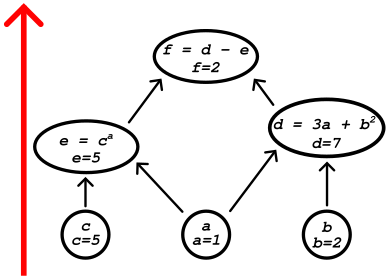
\includegraphics[width=\linewidth]{backprop_graph_combined_forward}
    \captionof{figure}{Прямой проход вычислительного графа.}
    \label{fig:backprop_graph_combined_forward}
\end{minipage}
\hfill
\begin{minipage}{0.45\textwidth}
    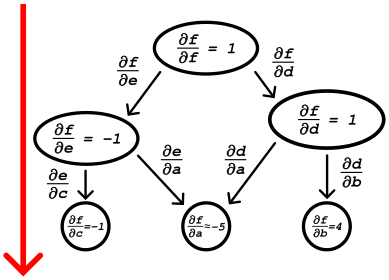
\includegraphics[width=\linewidth]{backprop_graph_combined_backward}
    \captionof{figure}{Обратный проход вычислительного графа.}
    \label{fig:backprop_graph_combined_backward}
\end{minipage}\\

Таким образом, всего за два прохода (прямой и обратный), мы можем 
найти производные желаемой функции, относительно всех ее составляющих. 
Если бы мы воспользовались дифференцированием прямого распространения 
(forward-mode differentiation), то получили бы производные всех составляющих 
по одной выбранной переменной (например: 
$\frac{\partial f}{\partial a}, \frac{\partial e}{\partial a}, 
\frac{\partial d}{\partial a}, \frac{\partial a}{\partial a}, 
\frac{\partial b}{\partial a}, \frac{\partial c}{\partial a}$), 
что тоже иногда применимо, но в нашем случаем потребовало бы еще 5ти вызов 
для расчета градиента функции $f$, что звучит как немного, но если 
вспомнить, что в глубоком обучении мы обычно имеем дело с функциями 
миллионов и миллиардов переменных, то выигрыш 1 000 000 000 vs 1 (если не брать в расчет 
прямое распространение) звучит неплохо.

\paragraph{4 фундаментальных уравнения метода обратного распространения ошибки}

До сих пор мы рассматривали логику работы backprop-а на примере функции 
3х переменных. Однако теперь, когда мы интуитивно понимаем как работает метод, 
рассмотрим его с более формальной стороны уже на примере нейронной сети. 

Для начала определим обозначения, которые позволят нам однозначно ссылаться на 
элементы в сети:
\begin{itemize}
    \item $w_{jk}^l$ - вес (weight) связи $k$-го нейрона в $(l-1)$-м слое и $j$-го нейрона в $l$-м слое.
    \item $b_j^l$ - смещение (bias) $j$-го нейрона в $l$-м слое.
    \item $a_j^l$ - активация (activation) $j$-го нейрона в $l$-м слое.
\end{itemize}

\def\layersep{3cm}
\begin{center}
    \begin{tikzpicture}[scale=1.2, transform shape, shorten >=1pt,->,draw=black!50,node distance=\layersep]
        % base neuron style: bigger, no fill, black outline
        \tikzstyle{neuron}         =[circle, draw=black, fill=none, minimum size=25pt, inner sep=0pt]
        \tikzstyle{input neuron}   =[neuron]
        \tikzstyle{hidden neuron}  =[neuron]
        \tikzstyle{output neuron}  =[neuron]
        \tikzstyle{annot}          =[text width=4em, text centered]
    
        % Input layer: 4 nodes
        \foreach \i in {1,...,4}
            \node[input neuron] (I-\i) at (0,{1.5cm-(\i-1)*1cm}) {};
    
        % Hidden layer: 5 nodes (4th labeled b_4^2)
        \foreach \i in {1,2,3,5}
            \node[hidden neuron] (H-\i) at (\layersep,{2cm-(\i-1)*1cm}) {};
        \node[hidden neuron] (H-4) at (\layersep,{2cm-(4-1)*1cm}) {$b_4^2$};
    
        % Output layer: 2 nodes (1st labeled a_1^3)
        \node[output neuron] (O-1) at (2*\layersep,{0.5cm}) {$a_1^3$};
        \node[output neuron] (O-2) at (2*\layersep,{-0.5cm}) {};
    
        % Connections: input → hidden
        \foreach \i in {1,...,4}
            \foreach \h in {1,...,5}
                \draw (I-\i) -- (H-\h);
    
        % Connections: hidden → outputs
        \foreach \h in {1,...,5}
            \foreach \o in {1,2}
                \draw (H-\h) -- (O-\o);
    
        % Special edge (H-4) → (O-1) drawn in solid black
        \draw[->,draw=black,line width=1.5pt] (H-4) -- node[midway,above,yshift=1pt] {$w_{14}^3$} (O-1);
    
        % Annotate the layers
        \node[annot,above of=H-1, node distance=1cm] (hl) {слой 2};
        \node[annot,left of=hl] {слой 1};
        \node[annot,right of=hl] {слой 3};
    \end{tikzpicture}
    
    \captionof{figure}{Схема нейронной сети с 3мя слоями и выделенными: 
    смещением $b_4^2$ (2й слой, 4й узел), выходным значением $a_1^3$ 
    (3й слой, 1й узел) и гранью, соединяющие эти два узла $w_{14}^3$.}
    \label{fig:nn_schematic}
\end{center}

Активацию мы получаем после применения функции активации $f$ к результату 
взешенной активации предыдщего слоя:
\begin{equation*}
    a_j^l \defeq f \left( \sum_k w_{jk}^l a_k^{l-1} + b_j^l \right),
\end{equation*}
где сумма происходит по всем нейронам $k$ в слое $(l-1)$. 

Также заведем еще одну переменную $z$ для взвешенной активации:
\begin{equation*}
    z_j^l \defeq \sum_k w_{jk}^l a_k^{l-1} + b_j^l.
\end{equation*}
А под $C$ будем понимать функцию стоимости.

Backprop - это про понимание того как изменение весов и смещений в сети 
влияет на изменение функции стоимости. В конечном итоге всё сводится 
к вычислению частных производных $\frac{\partial C}{\partial w_{jk}^l}$ и 
$\frac{\partial C}{\partial b_j^l}$. Но чтобы их посчитать, нам надо 
сперва ввести промежуточное значение $\delta_j^l$, которое мы будем звать 
ошибкой $j$-го нейрона в $l$-м слое. Backprop даст нам процедуру вычисления этой 
ошибки $\delta_j^l$, с помощью которой потом мы уже сможем найти 
$\frac{\partial C}{\partial w_{jk}^l}$ и $\frac{\partial C}{\partial b_j^l}$.

Определим ошибку как:
\begin{equation*}
    \delta_j^l \defeq \cfrac{\partial C}{\partial z_j^l}.
\end{equation*}
(В целом мы бы могли определить ошибку и как $\frac{\partial C}{\partial a_j^l}$. 
Вообще говоря, если так сделать, то все получится очень похоже на наши вычисления 
ниже, просто они станут немного алгебраически сложнее, так что будем использовать 
определение выше).

В основе backprop лежат 4 фундаментальных уравнения. С помощью них, мы сможем 
вычислить как ошибку $\delta_j^l$, так и градиент функции стоимости. Выведем же их 
(далее будет приведен упрощенный вывод фундаментальных уравнений, поскольку 
оригинальный вывод несколько сложнее, длинее и в конечном итоге сводится к нашему. 
Оригинальный вывод см. в \cite{backprop}).\\

\noindent\textbf{Уравнение ошибки выходного слоя, $\delta^L$:}

Воспользовавшись правилом дифференцирования сложной функции, 
перепишем выражение для нашей ошибки в терминах частных производных 
по активациям:

\begin{equation*}
    \delta_j^L \defeq \cfrac{\partial C}{\partial z_j^L} = 
    \sum_k \cfrac{\partial C}{\partial a_k^L} \cfrac{\partial a_k^L}{\partial z_j^L}, 
\end{equation*}
где сумма происходит по всем нейронам выходного слоя. 

Вспомним, что $a_k^L \defeq f(z_k^L)$, тогда
выражение $\cfrac{\partial a_k^L}{\partial z_j^L}$ имеет смысл только когда $k=j$, 
тк при $k \neq j$, $a_k^L$ не зависит от $z_j^L$. А значит, мы можем упростить 
выражение:
\begin{equation*}
    \delta_j^L = \cfrac{\partial C}{\partial a_j^L} \cfrac{\partial a_j^L}{\partial z_j^L} 
    = \cfrac{\partial C}{\partial a_j^L} \cdot f'(z_j^L).
\end{equation*}

Это и есть наше искомое первое уравнение. Перепишем его в матричном виде:
\begin{equation}
    \delta^L = \nabla_a C \odot f'(z^L).
    \tag{I}
\end{equation}
Здесь и далее, $\delta^L$ - вектор ошибок в слое $L$, 
$\nabla_a C$ - вектор, чьи компоненты это частные производные 
$\frac{\partial C}{\partial a_j^L}$, а $\odot$ означает произведение Адамара.\\

\noindent\textbf{Уравнение ошибки в терминах ошибки следующего слоя:}

Как и в прошлый раз, перепишем выражение для нашей ошибки, однако на этот раз, 
в терминах частных производных по взвешенным активациям следующего слоя:
\begin{equation*}
    \delta_j^l \defeq \cfrac{\partial C}{\partial z_j^l} = 
    \sum_k \cfrac{\partial C}{\partial z_k^{l+1}} \cfrac{\partial z_k^{l+1}}{\partial z_j^l}.
\end{equation*}
где сумма происходит по всем нейронам следующего слоя. 

Воспользовавшись нашим определением ошибки перепишем уравнение в виде:
\begin{equation}
    \delta_j^l = 
    \sum_k \cfrac{\partial C}{\partial z_k^{l+1}} \cfrac{\partial z_k^{l+1}}{\partial z_j^l} = 
    \sum_k \delta_k^{l+1} \cfrac{\partial z_k^{l+1}}{\partial z_j^l}
\end{equation}

Теперь вспомним, что $z_k^{l+1} \defeq \sum_i w_{ki}^{l+1} a_i^l + b_k^{l+1};\hspace{5pt} a_i^l \defeq f(z_i^l)$, тогда:
\begin{equation*}
    \cfrac{\partial z_k^{l+1}}{\partial z_j^l} = \sum_i w_{ki}^{l+1} \cfrac{\partial a_i^l}{\partial z_j^l},
\end{equation*}

где 
\begin{equation*}
    \cfrac{\partial a_i^l}{\partial z_j^l} = \begin{cases}
        0, \quad i \neq j \\
        f'(z_j^l), \quad i = j
    \end{cases}
\end{equation*}

Тогда
\begin{equation*}
    \cfrac{\partial z_k^{l+1}}{\partial z_j^l} = w_{kj}^{l+1} f'(z_j^l).
\end{equation*}

Подставляя в (1):
\begin{equation*}
    \delta_j^l = \sum_k \delta_k^{l+1} w_{kj}^{l+1} f'(z_j^l) = f'(z_j^l) \sum_k w_{kj}^{l+1} \delta_k^{l+1}
\end{equation*}

Это и есть наше искомое второе уравнение. Перепишем его в матричном виде:
\begin{equation*}
    \delta^l = ((W^{l+1})^T \delta^{l+1}) \odot f'(z^l),
    \tag{II}
\end{equation*}
где $(W^{l+1})^T$ означает транспонированную матрицу веса 
(элементы матрицы веса $W^l$ слоя $l$ это веса, соединяющие с $l$-м слоем нейронов, 
т.е. элемент $j$-го ряда и $k$-го столбца нашей матрицы это $w_{jk}^l$).

Объединяя уравнения (I) и (II), мы можем вычислить ошибку $\delta^l$ для любого 
слоя в нашей сети. Начинаем с (I) для вычисления $\delta^L$, затем применяем 
уравнение (II) для вычисления $\delta^{L-1}$, а затем снова уравнение (II) для 
вычисления $\delta^{L-2}$ и так далее.\\

\noindent\textbf{Уравнение для скорости изменения функции стоимости относительно смещения:}

Опять же перепишем выражение для нашей ошибки, но в терминах частных производных 
по смещениям:
\begin{equation*}
    \delta_j^l \defeq \cfrac{\partial C}{\partial z_j^l} = 
    \cfrac{\partial C}{\partial b_j^l} \cfrac{\partial b_j^l}{\partial z_j^l}.
\end{equation*}

вспоминая, что $z_j^l \defeq \sum_k w_{jk}^l a_k^{l-1} + b_j^l$:
\begin{equation*}
    \cfrac{\partial b_j^l}{\partial z_j^l} = 
    \left( \cfrac{\partial b_j^l}{\partial z_j^l} \right)^{-1} = 1
\end{equation*}

Тогда:
\begin{equation*}
    \delta_j^l = \cfrac{\partial C}{\partial b_j^l}.
    \tag{III}
\end{equation*}

Это и есть наше искомое третье уравнение.\\

\noindent\textbf{Уравнение для скорости изменения функции стоимости относительно веса:}

Распишем что мы хотим найти:
\begin{equation}
    \cfrac{\partial C}{\partial w_{jk}^l} = \sum_m \cfrac{\partial C}{\partial z_m^l} \cfrac{\partial z_m^l}{\partial w_{jk}^l} = \cfrac{\partial C}{\partial z_j^l} \cfrac{\partial z_j^l}{\partial w_{jk}^l}
\end{equation}

Вспоминаем, что $z_j^l \defeq \sum_i w_{ji}^l a_i^{l-1} + b_j^l$, тогда:
\begin{equation*}
    \cfrac{\partial z_j^l}{\partial w_{jk}^l} = \sum_i \cfrac{\partial}{\partial w_{jk}^l} w_{ji}^l a_i^{l-1} = \begin{cases}
        a_k^{l-1}, \quad i=k \\
        0, \quad i \neq k
    \end{cases}
\end{equation*}

Подставляя в (2):
\begin{equation*}
    \cfrac{\partial C}{\partial w_{jk}^l} = a_k^{l-1} \delta_j^l.
    \tag{IV}
\end{equation*}

Таким образом мы получаем наше четвертое и последнее фундаментальное 
уравнение метода обратного распространения ошибки. 

Объединим их: \\

\begin{mdframed}[
    userdefinedwidth=0.7\textwidth,
    align=center,
    frametitle={Fundamental Backpropagation Equations},
    frametitlealignment=\centering,  % Center the title
    innertopmargin=-1em,              % Decrease space between title area and equations
    innerbottommargin=7pt,           % Space below the last equation
    innerleftmargin=10pt,            % Padding on the left of content
    innerrightmargin=10pt,           % Padding on the right of content
    frametitleaboveskip=1em,         % Space above title text (within title bar)
    frametitlebelowskip=2pt,         % Space below title text (within title bar) before content
    % Optional styling:
    % roundcorner=5pt,
    % linewidth=1pt,
    % linecolor=blue,
    % backgroundcolor=blue!10,
]
    \begin{flalign*}
        &\delta^L = \nabla_a C \odot f'(z^L) && \text{(I)}&\\[0.5em]
        &\delta^l = ((W^{l+1})^T \delta^{l+1}) \odot f'(z^l) && \text{(II)}&\\[0.5em]
        &\cfrac{\partial C}{\partial b_j^l} = \delta_j^l && \text{(III)}&\\[0.5em]
        &\cfrac{\partial C}{\partial w_{jk}^l} = a_k^{l-1} \delta_j^l && \text{(IV)}&
    \end{flalign*}
\end{mdframed}

Объединяя теперь с алгоритмом обучения, например стохастическим градиентным 
спуском c мини-пакетом (mini-batch) размера $m$, получим упрощенную версию 
алгоритма расчета градиента функции стоимости \cite{NN_Nielsen}:
\begin{enumerate}
    \item \textbf{Ввод набора обучающих примеров}
    \item \textbf{Для каждого обучающего примера $x$:} Установить соответствующую входную активацию $a^{x,1}$, и выполнить следующие действия:
    \begin{itemize}
        \item \textbf{Прямое распространение:} Для каждого $l=2,3,...,L$ вычислить \\$z^{x,l}=W^l a^{x,l-1} + b^l$ и $a^{x,l} = f(z^{x,l})$. 
        \item \textbf{Ошибка выходного слоя $\delta^{x,L}$:} Вычислить вектор\\ $\delta^{x,L}=\nabla_a C_x \odot f'(z^{x,L})$.
        \item \textbf{Обратное распространение ошибки:} Для каждого $l=L-1, L-2, ..., 2$ вычислить \\$\delta^{x,l}=((W^{l+1})^T \delta^{x,l+1}) \odot f'(z^{x,l})$.
    \end{itemize}
    \item \textbf{Градиентный спуск:} Для каждого $l=L,L-1,...,2$ обновить веса по правилу\\$W^l \rightarrow W^l - \frac{\eta}{m} \sum_x \delta^{x,l} (a^{x,l-1})^T$\\и смещения по правилу\\$b^l \rightarrow b^l - \frac{\eta}{m} \sum_x \delta^{x,l}$.
\end{enumerate}
